\chapter{Обзор технологии LTE} \label{chapt5}

\section{Архитектура базовой станции} \label{section5_1}
Ключевым элементом сети LTE, отвечающим за эффективное использование частотного спектра, является базовая станция. В данном разделе представлена архитектура базовой станции и рассмотрены компоненты, участвующие в процессе управления ресурсами.

\begin{figure}[ht] 
  \center
  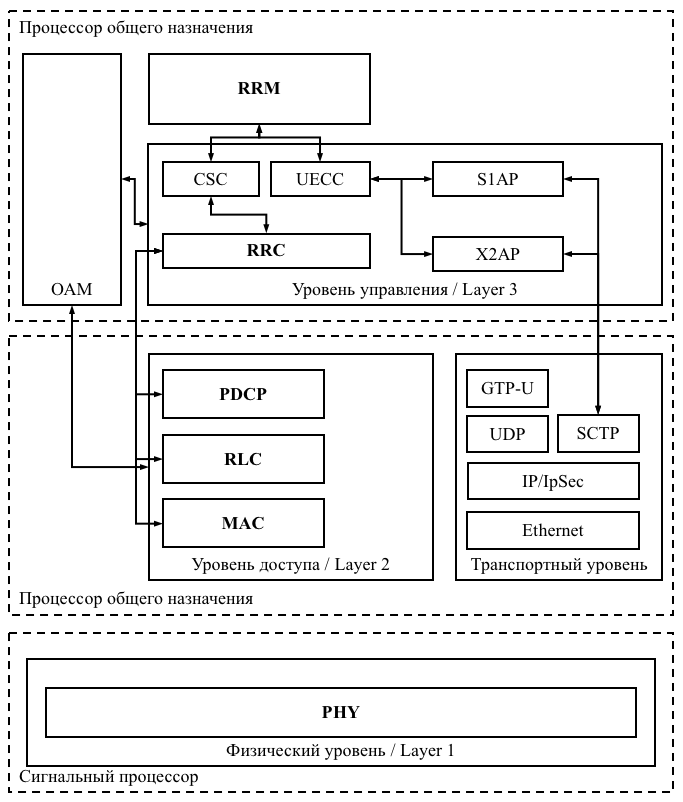
\includegraphics {image7}
  \caption{Архитектура базовой станции LTE. Источник \cite{Aricent}} 
  \label{img:image7}  
\end{figure}


Протокол PDCP (Packet Data Convergence Protocol) обеспечивает компрессию заголовков (ROHC), шифрование, сохранение порядка следования пакетов.

Протокол RLC (Radio Link Control) выполняет функции сегментирования, отброса дубликатов и сохранение порядка следования пакетов \cite{access2008and}. RLC функционирует в одном из трех режимов передачи: прозрачный (transparent mode, TM), передача без подтверждения (unacknowledged mode, UM) и передача с подтверждением (acknoledged mode, AM). В режиме AM поддерживаются специальные функции для повторной передачи данных.

Протокол RRC покрывает следующие функциональные области: передача системной информации, управление RRC соединением (RRC connection control). Сюда относятся процедуры создания, изменения и удаления RRC соединения, пейджинг, активацию защиты соединения, контроль ресурсов для передачи пользовательских данных. Также к этой области относится процедура хэндовера (handover) и конфигурация более низких уровней (PDCP, RLC, MAC).

Протокол RRC также осуществляет настройку измерений качества канала и отчетность на стороне пользовательского устройства, включая настройку и активацию периодов измерений (см. раздел \ref{section5_3}). Актуальность информации о состоянии канала напрямую влияет на эффективность передачи пользовательских данных.

Задача управления радиоресурсами решается протоколом RRM (Radio Resource Management). Сюда входит динамическое распределение ресурсов в восходящих и нисходящих направлениях, принятие решений о необходимости хэндовера и допуска пользователей к обслуживанию. Блок RRM также отвечает за ограничение использования спектра с целью контроля интерференции между базовыми станциями.

Задача протокола MAC (Media Access Control) заключается в выделении пользователям частотно временных ресурсов и поддержании гарантий качества обслуживания. Блок MAC также осуществляет выбор сигнально-кодовой конструкции, используемой для обслуживания пользователей.

\section{Физический уровень LTE} \label{section5_2}

Обмен между базовой станцией и абонентским устройством осуществляется кадрами (в терминологии LTE – радиокадр) длительностью 10 мс (см. рис. \ref{img:image8}). Стандарт предусматривает две структуры кадров. Одна для случая частотного разделения каналов (Frequency Division Duplex — FDD), другая - для временного (Time Division Duplex — TDD).

В LTE используется OFDM модуляция, хорошо исследованная при разработке систем DVB, Wi-Fi и WiMAX..В стандарте LTE установлен стандартный шаг между поднесущими ∆f = 15 кГц, что соответствует длительности OFDM-символа 66,7 мкс.

Все временные параметры в спецификации LTE привязаны к минимальному временному кванту !!   =  1/(2048 ∙ ∆!), где ∆! – шаг между поднесущими, стандартно – 15 кГц. Таким образом, длительность радиокадра – 307200 ∙ !!. Отметим, что квант времени соответствует тактовой частоте 30,72 МГц, что кратно стандартной в 3G-
системах частоте обработки 3,84 МГц (8×3,84 = 30,72) \cite{access2010lte}.

\begin{figure}[ht] 
  \center
  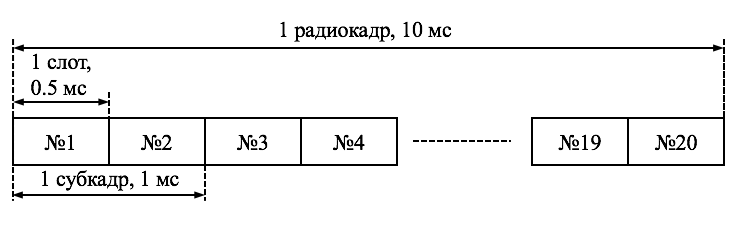
\includegraphics {image8}
  \caption{Структура кадра LTE. Источник \cite{вишневский2009технология}} 
  \label{img:image8}  
\end{figure}


В каждом слоте абонентскому устройству назначается определенный диапазон канальных ресурсов в частотно-временной области – ресурсная сетка (см. рис. \ref{img:image9}). Ячейка ресурсной сетки (ресурсный элемент) соответствует одной поднесущей в частотной области и одному OFDM-символу – во временной. Группа ресурсных элементов образует ресурсный блок. Ресурсный блок – это минимальный квант радиоресурса, выделяемый абонентскому устройству планировщиком базовой станции. Ресурсный блок занимает 12 поднесущих (т.е. 180 кГц) и 7 или 6 OFDM- символов, в зависимости от типа циклического префикса – так, чтобы общая длительность слота составляла 0,5 мс. Число ресурсных блоков в ресурсной сетке зависит от ширины полосы канала и составляет от 6 до 100 (ширина частотных полос восходящего/нисходящего каналов в LTE – от 1,4 до 20 МГц). В новой версии стандарта LTE-A добавлена возможность агрегации до 5 полос шириной 20 МГц \cite{access2013lte}. О распределении ресурсов в каждом слоте базовая станция сообщает в управляющем канале, располагающемся в начале каждого субкадра.

\begin{figure}[ht] 
  \center
  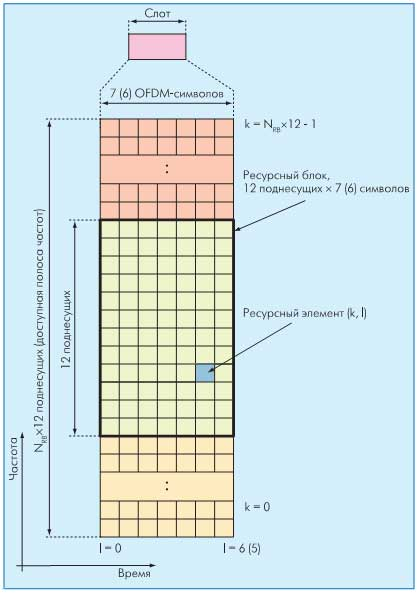
\includegraphics {image9}
  \caption{Ресурсная сетка LTE при стандартном шаге поднесущих ∆f = 15 кгц. Источник \cite{вишневский2009технология}} 
  \label{img:image9}  
\end{figure}

Поднесущие модулируются посредством 4-, 16- и 64-позиционной квадратурной фазово-амплитудной модуляции (QPSK, 16-QAM или 64-QAM). Соответственно, один символ на одной поднесущей содержит 2, 4 или 6 бит информации. При стандартном префиксе символьная скорость составит 14000 символов/с. Сигнал с полосой 20 МГц содержит 100 ресурсных блоков или 1200 поднесущих, что дает общую скорость в канале от 33,6 до 100,8 Мбит/с.

Для повышения надежности передачи на физическом уровне стандарт LTE использует механизм HARQ (Hybrid Automatic Repeat Request). HARQ представляет собой комбинацию высокоскоростного помехоустойчивого кода и стандартного механизма ARQ \cite{access2008and}. Эта технология позволяет пользовательскому устройству запросить дополнительные проверочные биты при обнаружении ошибки декодирования.

\section{Оценка канала} \label{section5_3}

Для эффективного осуществления передачи данных базовая станция должна иметь оценку качества канала до обслуживаемого пользователя. Эта оценка используется для планирования расписания передач. Стандарт LTE предусматривает возможность запросить у пользователя отчет с оценкой качества канала. Для того чтобы задать формат отчетов о качестве канала, базовая станция посылает пользователю служебное сообщение RRC ConnectionReconfiguration \cite{access2012lte} с указанием следующих параметров:

При получении сообщения RRC ConnectionReconfiguration \cite{access2012lte} пользовательское устройство проводит измерения мощности пилотных сигналов соседних станций и через время равное reportInterval посылает их в отчете Measurement report. Эти величины называются RSRP (Reference Signal Received Power) \cite{access2010lte} и квантуется в соответствии с рисунком 10.


